\section{White noise}

White noise is characterized as a sequence of independent identically distributed random variables, exhibiting the following properties:
\begin{itemize}
    \item The probability distribution remains constant across all times, indicating stationarity.
    \item  Independence among variables implies zero correlation at different times.
\end{itemize}
It is commonly defined with an expected value of zero:
\[\mathbb{E}\left[v(t)\right]=0\]
And a covariance structured as:
\[\gamma(\tau)=
\begin{cases}
    0 \qquad \text{for } \tau \neq 0 \\
    \lambda^2 \qquad \text{for } = 0
\end{cases}\]
This formulation indicates that white noise is entirely unpredictable. 
Typically, white noise is expressed as:
\[v(\cdot) \sim WN(0,\lambda^2)\]
Or as white noise with a Gaussian distribution:
\[v(\cdot) \sim WGN(0,\lambda^2)\]
\begin{example}
    Let's analyze the process $v(t)=\eta(t)+c\eta(t-1)$, where $\eta(\cdot) \sim WN(0,\lambda^2)$. 
    First, let's calculate the expected mean value $\mu(t)$: 
    \[\mu(t)=\mathbb{E}\left[v(t)\right]=\mathbb{E}\left[v(t)=\eta(t)+c\eta(t-1)\right]=\underbrace{\mathbb{E}\left[\eta(t)\right]}_0 +c\underbrace{\mathbb{E}\left[\eta(t-1)\right]}_0=0\]
    Next, we find the covariance $\gamma(0)$:
    \begin{align*}
        \gamma(0)       &=\text{Var}\left[v(t)\right]
                        &=\mathbb{E}\left[\left(v(t)-0\right)^2\right] \\
                        &=\mathbb{E}\left[\left(\eta(t)+c\eta(t-1)\right)^2\right] \\
                        &=\mathbb{E}\left[\eta(t)^2+2c\eta(t)\eta(t-1)+c^2\eta(t-1)^2\right] \\
                        &=\mathbb{E}\left[\eta(t)^2\right] + \mathbb{E}\left[2c\eta(t)\eta(t-1)\right] + \mathbb{E}\left[c^2\eta(t-1)^2\right] \\
                        &=\underbrace{\mathbb{E}\left[\eta(t)^2\right]}_{\lambda^2}  + 2c\underbrace{\mathbb{E}\left[\eta(t)\eta(t-1)\right]}_{0} + c^2\underbrace{\mathbb{E}\left[\eta(t-1)^2\right]}_{\lambda^2}  \\
                        &=\left( 1+c^2 \right)\lambda^2
    \end{align*}
    It's important to note that since $\eta(\cdot)$ has a mean of zero, the expected mean between two different time instants is null.
    The $\gamma(0)$ function is constant. 
    Now, let's consider other time instants:
    \begin{align*}
        \gamma(t,t+1)   &=\mathbb{E}\left[\left(v(t)v(t+1)\right)^2\right] \\
                        &=\mathbb{E}\left[\left(\eta(t)+c\eta(t-1)\right)\left(\eta(t+1)+c\eta(t)\right)\right] \\
                        &=\mathbb{E}\left[\eta(t)\eta(t+1)+c\eta(t-1)\eta(t+1)+c\eta(t)^2+c^2\eta(t-1)\eta(t)\right] \\
                        &=\underbrace{\mathbb{E}\left[\eta(t)\eta(t+1)\right]}_{0}  + c\underbrace{\mathbb{E}\left[\eta(t-1)\eta(t+1)\right]}_{0}  + c\underbrace{\mathbb{E}\left[\eta(t)^2\right]}_{\lambda^2}  + c^2\underbrace{\mathbb{E}\left[\eta(t-1)\eta(t)\right]}_{0}  \\
                        &=c\lambda^2
    \end{align*}
    \begin{align*}
        \gamma(t,t+2)   &=\mathbb{E}\left[\left(v(t)v(t+2)\right)^2\right] \\
                        &=\mathbb{E}\left[\left(\eta(t)+c\eta(t-1)\right)\left(\eta(t+2)+c\eta(t+1)\right)\right] \\
                        &=\mathbb{E}\left[\eta(t)\eta(t+2)+c\eta(t-1)\eta(t+2)+c\eta(t)\eta(t+1)+c^2\eta(t-1)\eta(t+1)\right] \\
                        &=\underbrace{\mathbb{E}\left[\eta(t)\eta(t+2)\right]}_{0}  + c\underbrace{\mathbb{E}\left[\eta(t-1)\eta(t+2)\right]}_{0}  + c\underbrace{\mathbb{E}\left[\eta(t)\eta(t+1)\right]}_{0}  + c^2\underbrace{\mathbb{E}\left[\eta(t-1)\eta(t+1)\right]}_{0}  \\
                        &=0
    \end{align*}
    We find that both $\gamma(t,t+1)$ and $\gamma(t,t+2)$ are constants. 
    Also, all time instants after $t+2$ will have a covariance with $t$ equal to zero. 
    Thus, in formula, we have:
    \[\begin{cases}
        \gamma(0)=(1+c^2)\lambda^2 \\
        \gamma(1)=c\lambda \\
        \gamma(\tau)=0 \qquad \tau \geq 2 \\
    \end{cases}\]
    Graphically, we can illustrate two cases based on the sign of the constant $c$: 
    \begin{figure}[H]
        \centering
        \begin{subfigure}{0.49\textwidth}
            \centering
            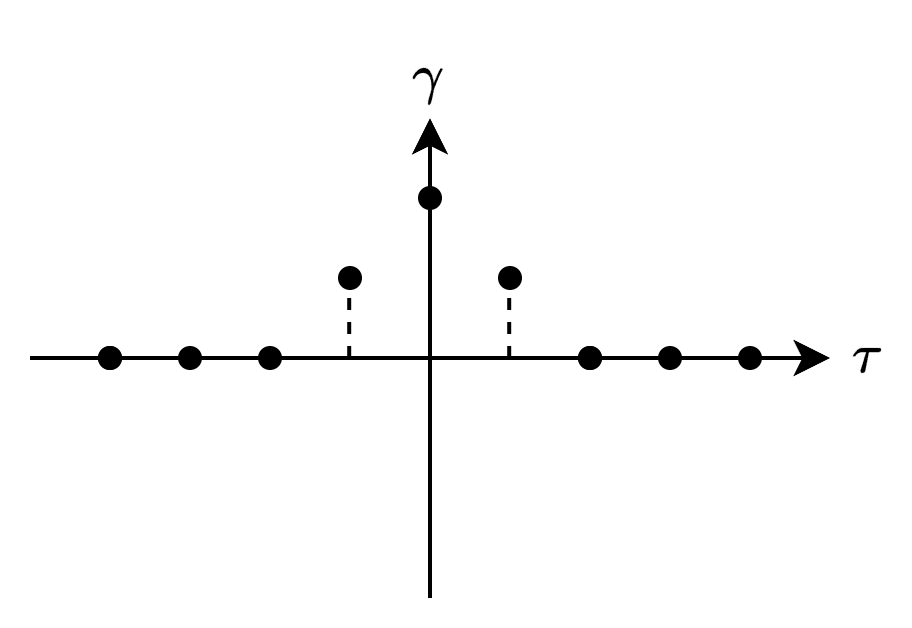
\includegraphics[width=0.75\linewidth]{images/cpos.png} 
            \caption{Positive constant $c$}
        \end{subfigure}
        \begin{subfigure}{0.49\textwidth}
            \centering
            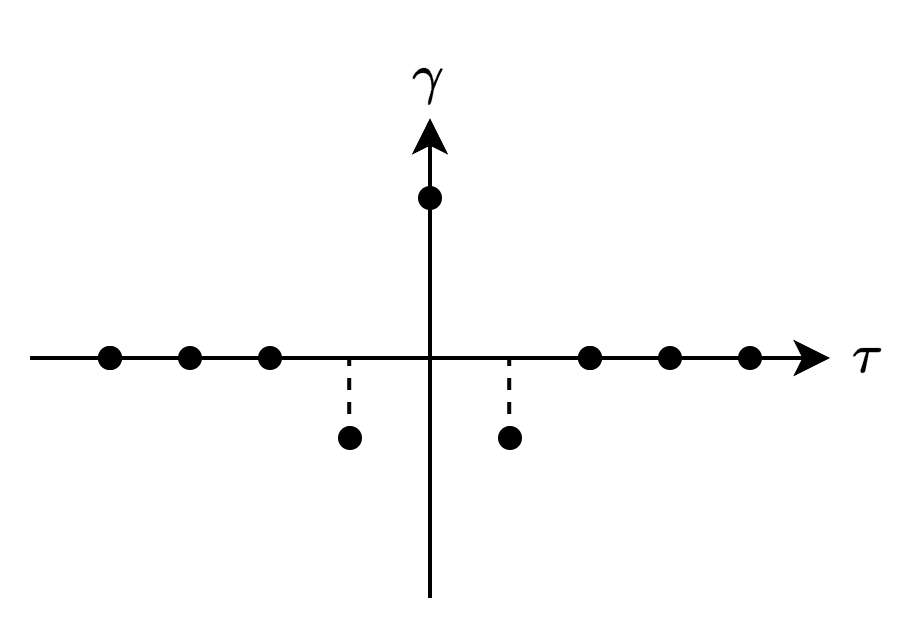
\includegraphics[width=0.75\linewidth]{images/cneg.png}
            \caption{Negative constant $c$}
        \end{subfigure}
        \caption{Possible values for the covariance}
    \end{figure}
\end{example}